\documentclass[conference]{IEEEtran}
\usepackage{amsmath,amssymb,amsfonts}
\usepackage{graphicx}
\usepackage{booktabs,multirow,array}
\usepackage{cite}
\usepackage{textcomp}
\usepackage{xcolor}
\usepackage{algorithm}
\usepackage{algpseudocode}
\usepackage{tikz}
\usetikzlibrary{arrows.meta,positioning,calc,fit,backgrounds}
\usepackage{balance}
\usepackage{placeins}
\usepackage{fontspec}
\setmainfont{Times New Roman}
\def\BibTeX{{\rm B\kern-.05em{\sc i\kern-.025em b}\kern-.08em T\kern-.1667em\lower.7ex\hbox{E}\kern-.125emX}}
\renewcommand{\algorithmicrequire}{\textbf{Input:}}
\renewcommand{\algorithmicensure}{\textbf{Output:}}
\newcommand{\ok}{\ensuremath{\checkmark}}
\newcommand{\part}{\ensuremath{\circ}}
\newcommand{\no}{--}

\makeatletter
\renewcommand\section{\@startsection{section}{1}{\z@}{1.5ex plus 1.5ex minus 0.5ex}{0.7ex}{\normalfont\centering\bfseries}}
\makeatother
\newcommand{\authbox}[2]{\begin{minipage}[t]{0.32\textwidth}\centering\fontsize{7.5}{9}\selectfont #1\\ Department of Computer Engineering,\\ Vishwakarma Institute of Technology,\\ Pune, India\\ #2\end{minipage}}

\renewcommand{\topfraction}{0.9}\renewcommand{\dbltopfraction}{0.9}\renewcommand{\bottomfraction}{0.8}\renewcommand{\textfraction}{0.1}\renewcommand{\floatpagefraction}{0.7}\renewcommand{\dblfloatpagefraction}{0.7}
\begin{document}

\title{Few-Shot Temporal Subgraph Anomaly Detection and Structure-Aware Anomaly Generation in Functional Brain Networks}

\author{%
\authbox{Dr. Prof. Premanand Ghadekar}{premanand.ghadekar@vit.edu}\hfill
\authbox{Harsh Patel}{patel.harsh24@vit.edu}\hfill
\authbox{Tanaya Hartalekar}{tanaya.hartalekar24@vit.edu}\\[1.6em]
\authbox{Hanil Shah}{hanil.shah24@vit.edu}\hspace{0.12\textwidth}
\authbox{Shravani Dixit}{shravani.dixit24@vit.edu}}

\maketitle

\noindent\textbf{\textit{Abstract:}} \textbf{\textit{Resting-state fMRI connectivity is usually analysed as one static graph per subject, which can hide localized changes in how brain substructures evolve, while labelled abnormal subjects are scarce. We study temporal subgraph anomaly detection. A weighted Graph Isomorphism Network (GIN) encodes stable, seed-centred subgraphs of sliding-window Pearson graphs, and a GRU trained only on control subjects predicts the next embedding; the prediction error, calibrated on held-out controls, is the anomaly score. A gradient-guided, PGD-style edit of existing edge weights of real control subgraphs generates synthetic anomalies, which are combined with 1, 5 or 10 real ASD subjects in a logistic-regression head. On ABIDE~I (871 subjects, 20 sites, subject-level 609/131/131 split) the detector does not separate ASD from control subjects (test AUROC 0.453, 95\% CI 0.353--0.552), and persistence and static embedding-distance baselines are also at chance. The generator produced 7,200 records without constraint violations; at high severity 45.8\% of structure-aware transitions exceed the control-calibrated threshold versus 4.8\% for random edits of equal budget, although this is measured with the model that guides the edit. Generated anomalies raise 1-shot F1 from 0.006 to 0.39, but AUROC stays near 0.50 and the F1 matches that of a random classifier flagging the same fraction of subjects. An exploratory estimate of ADOS-based severity bands from the same scores is no better than a majority-class baseline. The contribution is a reproducible formulation, a leakage-controlled protocol, and a documented negative result.}}

\medskip\noindent\textbf{\textit{Keywords:}} \textit{Functional brain networks, temporal graph learning, subgraph anomaly detection, graph isomorphism network, few-shot learning, autism spectrum disorder, resting-state fMRI.}

%=====================================================================
\section{INTRODUCTION}
Resting-state functional MRI (rs-fMRI) describes the brain as a graph whose nodes are regions of interest (ROIs) and whose edges quantify statistical dependence between ROI time series \cite{bullmore2009,smith2011}. Multi-site releases such as the Autism Brain Imaging Data Exchange (ABIDE) \cite{dimartino2014} have made it possible to apply graph neural networks (GNNs) to large cohorts, typically by classifying one connectivity graph per subject \cite{parisot2018,li2021braingnn,kan2022,cui2023}. Performance on ABIDE is modest and strongly affected by acquisition site \cite{abraham2017,heinsfeld2018,yu2018harm}.

Connectivity is not static: sliding-window analyses show that it fluctuates over tens of seconds \cite{hutchison2013,allen2014,preti2017}. Recent spatio-temporal GNNs model this variation, but they classify the whole scan from graph-level readouts \cite{kim2021,gadgil2020}. Two practical gaps remain. First, whole-graph readouts do not say \emph{which} brain substructure behaved unusually, or \emph{when}. Second, labelled abnormal subjects are scarce and diagnostic labels are only a weak proxy for abnormal connectivity dynamics. Normative modelling in neuroimaging addresses the second point by characterising each individual by deviation from a reference cohort \cite{marquand2016}; graph anomaly detection offers tools for scoring such deviations \cite{ma2023survey}.

This paper asks whether \emph{unusual temporal changes in localized connectivity substructures can be identified by learning normal temporal behaviour from control subjects, and whether a small number of ASD subjects, together with synthetically generated anomalies, helps adapt the detector.} The distinction from classification matters: a high anomaly score is a statement about deviation from a learned control distribution, not a diagnosis, and we make no clinical claim.

\textbf{Objectives.} (O1) Build a leakage-controlled pipeline from ROI time series to temporal subgraph embeddings. (O2) Learn control dynamics with a GRU and score transitions by prediction error. (O3) Calibrate thresholds on held-out controls. (O4) Generate synthetic anomalies grounded in the learned model and validate them. (O5) Evaluate few-shot adaptation against honest baselines.

\textbf{Research questions.} RQ1: does temporal modelling help over static scoring? RQ2: does subgraph localization help over whole-graph scoring? RQ3: does few-shot support (0/1/5/10 subjects) help? RQ4: are recurring anomalous subgraphs reproducible across support draws? RQ5: is the framework robust to window size, sparsification and subgraph size? RQ6: does it generalize across sites? RQ7: can the anomaly scores of ASD subjects estimate ADOS-based severity bands? Sections~\ref{sec:results} and~\ref{sec:discussion} state, for each, whether the evidence supports an answer; several are explicitly left unanswered.

\textbf{Contributions.} (i) A formulation of temporal subgraph transition anomaly scoring with stable subgraph tracking, a two-level threshold calibration, and subject-level aggregation. (ii) A complete implementation with subject-level isolation asserted in code, including the diagnosis of a multiple-comparisons failure (a single per-transition threshold flagged all 131 test subjects). (iii) A structure-aware, weight-only anomaly generator and its validation against a random baseline. (iv) An exploratory severity estimator linked to ADOS-2 calibrated severity scores \cite{gotham2009}, with its negative result. (v) An empirical study reporting negative and inconclusive results with confidence intervals, a chance-matched F1 diagnostic for few-shot evaluation, and a list of experiments still needed. GIN \cite{xu2019gin} and GRU \cite{cho2014} are used as components; we do not claim them as novel.

%=====================================================================
\section{LITERATURE REVIEW}
\subsection{Functional connectivity and dynamic connectivity}
Pearson and partial correlation are reliable estimators of ROI-pair dependence in simulation \cite{smith2011}, and brain graphs summarise them with graph-theoretic measures \cite{bullmore2009}. ROI definitions vary; for instance the HCP multimodal parcellation has 360 areas \cite{glasser2016}. Sliding-window estimates of time-varying connectivity reveal recurring whole-brain states \cite{allen2014}, with well-documented pitfalls in window length and interpretation \cite{hutchison2013,preti2017}.

\subsection{GNNs for brain networks}
Population-graph GCNs treat subjects as nodes \cite{parisot2018}; subject-level models include metric learning on connectomes \cite{ktena2017}, edge-aware convolutions \cite{kawahara2017}, interpretable ROI-aware GNNs \cite{li2021braingnn}, transformers \cite{kan2022} and a benchmark of design choices \cite{cui2023}, building on spectral GCNs \cite{kipf2017}. The Graph Isomorphism Network is as discriminative as the 1-WL test among message-passing GNNs \cite{xu2019gin}. All these works are supervised and operate on whole-scan graphs. Contrast subgraphs identify the subgraph whose density differs most between ASD and control groups, but at the group level and without a temporal model \cite{lanciano2020}.

\subsection{Temporal graph learning}
Dynamic-graph models include memory-based networks for event streams \cite{rossi2020tgn} and recurrent evolution of GCN weights across snapshots \cite{pareja2020}. For brain data, STAGIN applies a GIN per sliding window with attention readout and a Transformer over time to classify sex and task state on HCP \cite{kim2021}, and ST-GCN models short BOLD sub-sequences \cite{gadgil2020}; sliding-window tensor decomposition has been used for group-level aberrant dynamic connectivity in ASD \cite{aggarwal2019}. None predicts the next embedding of a tracked local subgraph to score anomalies.

\subsection{Graph anomaly detection}
Surveys organise deep graph anomaly detection by anomaly type (node, edge, subgraph, graph) and by static versus dynamic setting \cite{ma2023survey,pang2021review}. Reconstruction-error scoring on attributed networks \cite{ding2019dominant}, one-class objectives \cite{ruff2018}, graph-level distillation \cite{ma2022glocal}, and edge-anomaly models for dynamic graphs \cite{yu2018netwalk,zheng2019addgraph} are the closest methodological precedents. In brain data, control-only models for temporal multiplex networks \cite{behrouz2023} and temporal hypergraphs \cite{sadeghian2024} score edges or hyperedges with injected synthetic anomalies, and curvature has been used to flag critical edges in temporal correlation networks \cite{chatterjee2021}. In our reading these works do not track seed-centred subgraphs with a next-embedding predictor, do not generate anomalies by gradient-guided weight edits, and do not evaluate few-shot adaptation.

\subsection{Few-shot learning and synthetic anomalies}
Few-shot learning is surveyed in \cite{wang2021fewshot}, with meta-learning \cite{finn2017} and metric-based \cite{snell2017} methods. For graph anomalies, a few labelled anomalies can be exploited by cross-network meta-learning \cite{ding2021fewshot}, and deviation losses use a few labelled anomalies for anomaly scoring \cite{pang2019devnet}. Brain-network few-shot work is supervised: multi-task meta-learning on connectomes \cite{yang2022meta}, graph foundation models with prompts \cite{wei2025}, and few-shot ASD classification from structural MRI \cite{dhinagar2023}. Synthetic samples for graphs have been produced by embedding-space interpolation \cite{zhao2021smote} and by generative models \cite{chen2020gaan}. Gradient-based structure perturbation is well established in adversarial robustness \cite{zugner2018,dai2018,xu2019topology}, building on projected gradient descent (PGD) \cite{madry2018}; we reuse the idea constructively to generate anomalies, not to attack a classifier.

\subsection{Research gap}
Table~\ref{tab:lit} compares the closest works. After a targeted search (not exhaustive) we found no prior work that combines (a) tracked, localized brain subgraphs with next-embedding prediction, (b) gradient-guided edge-weight perturbation to synthesize anomalies, and (c) few-shot anomaly adaptation for ASD. Each ingredient exists separately, so our claim concerns the combination, to our knowledge, and its evaluation, not any single component.

\begin{table*}[!tp]
\caption{Comparison with closest prior work. \ok: addressed; \part: partially (see text); --: not addressed in the cited work as we read it. ``Loc.'' = localization below graph level.}
\label{tab:lit}
\centering\footnotesize
\setlength{\tabcolsep}{3pt}
\begin{tabular}{@{}>{\raggedright\arraybackslash}p{1.0cm}>{\raggedright\arraybackslash}p{3.8cm}>{\raggedright\arraybackslash}p{4.2cm}ccc >{\raggedright\arraybackslash}p{4.2cm}@{}}
\toprule
Ref. & Task / data & Method & Temporal & Loc. & Few-shot & Relation to this work / limitation \\
\midrule
\cite{parisot2018} & ASD, AD classification (ABIDE, ADNI) & Population-graph GCN & \no & \no & \no & Subjects as nodes; static, supervised \\
\cite{li2021braingnn} & fMRI classification (ABIDE I, HCP task) & ROI-aware GNN with ROI pooling & \no & \part & \no & Whole-scan graphs; supervised \\
\cite{kim2021} & Sex / task from dynamic FC (HCP) & GIN per window, attention readout, Transformer & \ok & \no & \no & Graph-level readout; HCP only \\
\cite{gadgil2020} & Sex / age (HCP, NCANDA) & Spatio-temporal GCN & \ok & \no & \no & Supervised regression/classification \\
\cite{lanciano2020} & ASD vs.\ control brain networks & Contrast subgraph (density difference) & \no & \ok & \no & Group-level, static \\
\cite{aggarwal2019} & ASD dynamic networks & Sliding-window tensor decomposition & \ok & \part & \no & Group statistics, no per-subject score \\
\cite{chatterjee2021} & ADHD temporal networks & Forman-Ricci curvature & \ok & \part & \no & No learning; no per-subject score \\
\cite{behrouz2023} & PD/ADHD/ASD anomaly detection & Temporal multiplex walks, control-only training & \ok & \part & \no & Edge-level; negative-sampling anomalies \\
\cite{sadeghian2024} & ASD/ADHD anomaly detection & Temporal hypergraph walks, control-only & \ok & \part & \no & Hyperedge-level; preprint \\
\cite{ding2021fewshot} & Static attributed networks & Cross-network meta-learning & \no & \part & \ok & Node anomalies; non-brain \\
\cite{yu2018netwalk,zheng2019addgraph} & Dynamic graph edge anomalies & Embedding / attention-GRU GCN & \ok & \part & \no & Non-brain; not few-shot \\
\cite{ma2022glocal} & Graph-level anomalies (static) & Glocal knowledge distillation & \no & \no & \no & One-class; no temporal model \\
\cite{xu2019topology} & GNN robustness & PGD topology attack & \no & \no & \no & Attack on classifiers, not anomaly generation \\
\cite{yang2022meta} & Brain connectomes, small data & Multi-task meta-learning & \no & \no & \ok & Static, supervised \\
This work & ASD vs.\ control (ABIDE I) & Stable subgraph GIN+GRU, generated anomalies & \ok & \ok & \ok & Evaluated honestly; see Sec.~\ref{sec:results} \\
\bottomrule
\end{tabular}
\end{table*}

%=====================================================================
\section{PROBLEM FORMULATION}
\label{sec:problem}
Let subject $s$ have an ROI time-series matrix $X^{(s)}\in\mathbb{R}^{N\times T_s}$ with $N{=}360$ ROIs and a diagnostic label $y^{(s)}\in\{0,1\}$ ($0$ control, $1$ ASD). Windows of length $L$ and stride $\sigma$ give $K_s=\lfloor (T_s-L)/\sigma\rfloor+1$ windows. For ROIs $i,j$ in window $k$ (indices $t\in\mathcal{W}_k$, $|\mathcal{W}_k|=L$),
\begin{equation}
r^{(k)}_{ij}=\frac{\sum_{t\in\mathcal{W}_k}(x_{it}-\bar{x}_i)(x_{jt}-\bar{x}_j)}{\sqrt{\sum_{t\in\mathcal{W}_k}(x_{it}-\bar{x}_i)^2\sum_{t\in\mathcal{W}_k}(x_{jt}-\bar{x}_j)^2}}.
\label{eq:pearson}
\end{equation}
Graph snapshot $G_k=(V,E_k,w^{(k)})$ has $V$ the $N$ ROIs and $E_k$ the $\lfloor\rho N(N{-}1)/2\rfloor$ pairs with largest $|r^{(k)}_{ij}|$; edge weights are the signed values $w^{(k)}_{ij}=r^{(k)}_{ij}$, edges are undirected (stored in both directions) and there are no self-loops. A seed set $\mathcal{V}_{\mathrm{seed}}\subset V$ defines, for $v\in\mathcal{V}_{\mathrm{seed}}$, a \emph{stable} 1-hop node set $V_v=\{v\}\cup\mathcal{N}_1(v;G_1)$ fixed at the first window, and the subgraph trajectory $S_v^{(k)}=G_k[V_v]$, $k=1,\dots,K_s$. An encoder $f_\theta$ yields $z^{(k)}_v=f_\theta(S^{(k)}_v)\in\mathbb{R}^{D}$, and a predictor $g_\phi$ yields $\hat z^{(k+1)}_v=g_\phi(z^{(1)}_v,\dots,z^{(k)}_v)$. The transition anomaly score is
\begin{equation}
A^{(k)}_v=\bigl\|z^{(k+1)}_v-\hat z^{(k+1)}_v\bigr\|_2 .
\label{eq:score}
\end{equation}
\emph{Task.} Given control subjects only to fit $(f_\theta,g_\phi)$, held-out controls to calibrate thresholds, and optionally $K$ ASD support subjects, produce (a) a subject-level score and decision, and (b) the set of flagged $(v,k)$ pairs. The positive class for evaluation is ASD, the evaluation unit is the subject, and no transition-level ground truth exists.

\emph{Assumptions.} Prediction error is a valid anomaly indicator only if (A1) the encoder preserves information about connectivity strength, (A2) the predictor does not simply copy the previous embedding or collapse, (A3) the control calibration set is exchangeable with unseen normal data, and (A4) abnormal connectivity dynamics in ASD, if present, are not smaller than the within-control variability. A4 is empirical and, as Sec.~\ref{sec:results} shows, is not supported here. Correlation strength, graph structure, embedding-space error, statistical significance and clinical meaning are distinct quantities and are not conflated.

%=====================================================================
\section{PROPOSED METHODOLOGY}
\label{sec:method}
Figure~\ref{fig:pipeline} summarises the implemented pipeline. \emph{Status:} stages A--J below are implemented and were run; the few-shot recurrence statistic is implemented and evaluated; a support-weighted score and anatomical labelling of ROIs are \emph{not} implemented; subject-level anomaly ``signatures'' exist as lists of flagged (subject, seed ROI, transition, score) records without anatomical labels.

\begin{figure*}[!tp]
\centering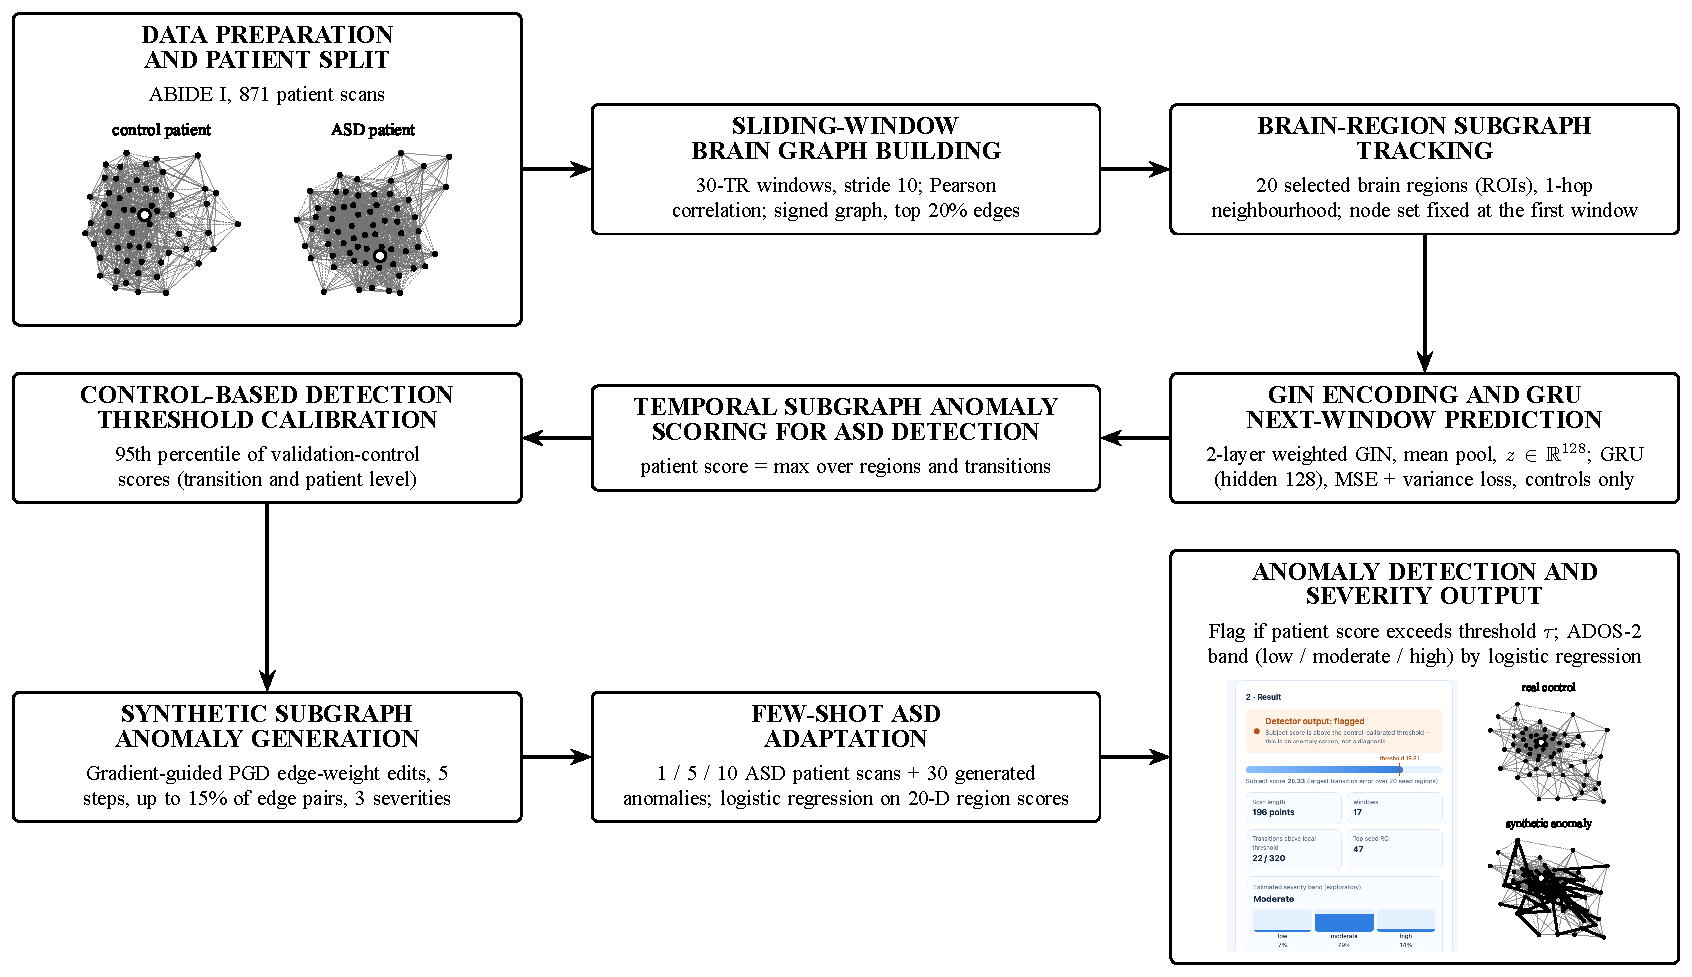
\includegraphics[width=\textwidth]{figures/fig_flow_compact.pdf}
\caption{End-to-end pipeline, read left to right on rows 1 and 3 and right to left on row 2. Example images: brain-region subgraphs of a control and an ASD test scan (input, first window; nodes are brain regions, edges are strongest correlations), and for the output a screenshot of the demo application with a real control subgraph and its synthetic anomaly (edited edges drawn bold). Test scans are used only at the final detection step.}
\label{fig:pipeline}
\end{figure*}

\subsection{Dataset and preprocessing}
We use ABIDE~I \cite{dimartino2014} ROI time series with 360 ROIs and variable scan length. According to the extraction script distributed with the release \cite{brahim2020}, the series come from the preprocessed ABIDE (CPAC pipeline, band-pass filtering, global signal regression, quality-checked subjects only), parcellated with the Glasser 360-area atlas \cite{glasser2016} using Nilearn \cite{abraham2014}; the exact filter cut-offs are not recorded in our project files. The cohort has 871 subjects (403 ASD, 468 typical controls, 20 sites). Re-applying the quality filter to the ABIDE phenotype file reproduces exactly this cohort size and the ASD/control count at all 20 sites. Site effects and demographic covariates are not modelled (see Sec.~\ref{sec:discussion}). Splits are drawn at the subject level, stratified by diagnosis (seed 42), giving 609 train (328 control, 281 ASD), 131 validation (70/61) and 131 test (70/61) subjects. Only the 328 train-control subjects fit the encoder and predictor; the 70 validation controls calibrate thresholds; the 281 train-ASD subjects form the support pool; the 131 test subjects are used only for final evaluation. Disjointness of the support set from validation and test subjects is checked in code before every support-set draw (a violation raises an error).

\subsection{Sliding-window connectivity and graph construction}
Eq.~(\ref{eq:pearson}) is evaluated per window with $L{=}30$ TR and stride $\sigma{=}10$ TR, giving 5--29 windows per subject (mean 16.7). In each window the $\lfloor 0.2\cdot 64{,}620\rfloor=12{,}924$ pairs with largest $|r|$ are retained (25,848 directed edges), keeping the sign of $r$; the diagonal is excluded, so there are no self-loops. Negative correlations are therefore kept as negative edge weights, not discarded. Only the sparsified graphs are persisted (1.4~GB for all subjects); the dense matrices are discarded after thresholding.

\subsection{Candidate subgraphs and stable tracking}
Whole 360-node graphs are too large to model per window and do not localize anomalies. Using $k{=}1$ neighbourhoods around all 360 ROIs gives 5.25 million subgraphs for the cohort (about 114~GB uncompressed), so training uses a deterministic, stratified subsample of 20 seed ROIs (selection seed 42), cached once. The mean subgraph has 71.1 nodes (median 69; 5th--95th percentile 28--121; range 1--176), where a 1-node subgraph is an isolated seed. \emph{Tracking.} Letting the node set follow each window's neighbourhood (dynamic tracking) gave a mean consecutive-window Jaccard similarity of 0.378 in a six-subject pilot, so the node set is instead fixed at the first window (stable tracking); only edges and weights vary. This makes $S_v^{(k)}$ a fixed set of ROIs observed repeatedly. It does not make the edge set fixed: the sparsification is per window, and the mean Jaccard similarity of the edge sets of consecutive windows is 0.435 (60 randomly drawn subjects $\times$ 20 seeds), so edge presence is itself a substantial source of temporal change. Windows with no valid data do not occur in the cached cohort (every subject has $\geq5$ windows); the correspondence problem for ROI sets that move across windows is sidestepped, not solved.

\subsection{GIN-based representation}
Node features are the constant $h_i^{(0)}{=}1$, so structure and edge weights carry all information. Each of two layers computes
\begin{equation}
h_i^{(l)}=\mathrm{ReLU}\!\Bigl(\mathrm{MLP}^{(l)}\bigl((1+\epsilon_l)h_i^{(l-1)}+\sum_{j\in\mathcal{N}(i)}w_{ij}h_j^{(l-1)}\bigr)\Bigr),
\label{eq:gin}
\end{equation}
with trainable $\epsilon_l$, an MLP of two linear layers (hidden width 64), and the signed edge weight $w_{ij}$ as a scalar message multiplier, which extends the unweighted GIN of \cite{xu2019gin}. The graph embedding is $z=W_o\,\frac{1}{|V_v|}\sum_i h_i^{(2)}+b_o\in\mathbb{R}^{128}$. GIN is chosen because it is maximally discriminative among message-passing GNNs \cite{xu2019gin}; it remains limited by constant input features, signed weights entering only linearly, and mean pooling, which discards subgraph size.

\subsection{GRU temporal prediction}
A single-layer GRU of hidden size 128 \cite{cho2014} reads $z^{(1)},\dots,z^{(k)}$ and a linear read-out gives $\hat z^{(k+1)}$ (Eq.~\ref{eq:score}); it is history-dependent. The encoder and GRU are trained jointly from random initialization on train-control subjects only:
\begin{equation}
\mathcal{L}=\underbrace{\tfrac{1}{B}\sum_{b}\tfrac{1}{(K_b-1)D}\sum_{k}\|\hat z_b^{(k+1)}-z_b^{(k+1)}\|_2^2}_{L_{pred}}+\lambda L_{var},
\label{eq:loss}
\end{equation}
\begin{equation}
L_{var}=\tfrac{1}{D}\sum_{d=1}^{D}\max\bigl(0,\,1-\sqrt{\mathrm{Var}_{\mathcal{B}}(z_d)+10^{-4}}\bigr),\quad \lambda=0.5 ,
\end{equation}
where $B$ is the number of (subject, seed) sequences per step and $\mathrm{Var}_{\mathcal{B}}$ is the variance over all embeddings in the batch. Because targets are produced by the encoder being trained, $L_{pred}$ alone has a trivial minimizer (a constant embedding); $L_{var}$ is a VICReg-style variance term \cite{bardes2022} that penalizes any dimension whose batch standard deviation falls below 1. Gradients flow through both the input and the target embeddings.

\subsection{Transition scoring and subject aggregation}
Eq.~(\ref{eq:score}) is computed for $k=1,\dots,K_s-1$ and every seed. Large errors indicate a transition the control-trained predictor did not anticipate; they are not a measure of severity or diagnosis. The subject score is the maximum over seeds and transitions,
\begin{equation}
S^{(s)}=\max_{v\in\mathcal{V}_{\mathrm{seed}}}\ \max_{k}\ A^{(k)}_v .
\label{eq:subject}
\end{equation}
The maximum is a design choice, not a validated one: it makes $S$ grow with the number of transitions, so scan length is a potential confound (Sec.~\ref{sec:results}); a mean over transitions is evaluated as a sensitivity check.

\subsection{Normal-subject calibration}
Two thresholds are calibrated from validation controls only, both at the 95th percentile $P_{95}$: $\tau_{tr}=P_{95}$ of all validation-control transition scores (21,760 transitions), and $\tau_{sub}=P_{95}$ of the 70 validation-control subject scores $S$. Calibration is global (shared across seeds). A single threshold $\tau_{tr}$ applied with an ``any transition'' rule is a multiple-comparisons error: with about 280 transitions per subject (20 seeds $\times\sim$14) a 5\% per-transition exceedance rate makes almost every subject cross it, and indeed flagged all 131 test subjects in our first attempt. $\tau_{tr}$ is therefore used only for localization, and $\tau_{sub}$, calibrated on the statistic actually thresholded, for subject decisions. We note that this diagnosis was made after seeing the test-set flag count, so operating-point metrics (precision, recall, F1) are not strictly blind to this design step; threshold-free metrics (AUROC, AUPRC) are unaffected.

\subsection{Few-shot ASD support and recurrence}
For $K\in\{1,5,10\}$, support subjects are drawn without replacement from the train-ASD pool (five independent draws per $K$, seeds 42--46). For seed ROI $v$, the recurrence statistic is
\begin{equation}
C(v)=\frac{1}{K}\sum_{j=1}^{K}\mathbf{1}\bigl[\max_k A^{(k)}_{v,j}>\tau_{tr}\bigr],
\label{eq:recurrence}
\end{equation}
the fraction of support subjects with at least one anomalous transition in subgraph $v$. High $C(v)$ would mark a \emph{shared} anomaly; a subject whose flags are absent from the other support subjects would carry an \emph{individual} one. An optional support-weighted score $A_{final}=A(1+\lambda C(v))$ was considered but is not implemented or evaluated, so we make no claim about it. Because Eq.~(\ref{eq:recurrence}) uses the same ``any transition'' flag discussed above, it requires a control null reference to be interpretable (Sec.~\ref{sec:results}).

\subsection{Structure-aware anomaly generation}
Anomalies are generated from real control subgraphs by editing only existing edge weights, so node identity, edge identity, symmetry and absence of self-loops are preserved by construction. For a train-control subject, seed $v$ and transition $t\to t{+}1$, let $\hat z=g_\phi(z^{(1)},\dots,z^{(t)})$ be the frozen predictor's causal estimate and $w$ the weights of the real $S_v^{(t+1)}$. With $\mathcal{J}(w)=\|f_\theta(S_v^{(t+1)};w)-\hat z\|_2^2$, the gradient $g_e=\partial\mathcal{J}/\partial w_e$ is computed for each directed edge and combined over the two directions of each undirected pair $p$: $g_p=\sum_{e\in p}g_e$. The $m=\max(1,\mathrm{round}(\alpha\rho_e|\mathcal{P}|))$ pairs with largest $|g_p|$ at the unmodified graph are selected ($\rho_e{=}0.15$, severity $\alpha\in[0,1]$), and $Q{=}5$ projected sign-gradient steps are taken, recomputing the gradient each time:
\begin{equation}
w_p^{(q+1)}=\mathrm{clip}_{[-1,1]}\!\Bigl(w_p^{(q)}+\tfrac{\alpha\,\delta_{\max}}{Q}\,\mathrm{sgn}\bigl(g^{(q)}_p\bigr)\Bigr),\quad \delta_{\max}{=}0.6 ,
\label{eq:pgd}
\end{equation}
applied identically to both directions of $p$ \cite{madry2018,xu2019topology}. A single large step overshot: on one held-out example the score at $\alpha=0.25,0.55,0.9$ was 5.28, 8.03, 5.03, which motivated five small steps. The random baseline edits $m$ uniformly chosen pairs by $\pm\alpha\delta_{\max}$ in one move, the same maximum displacement. The score of a generated record is $\|f_\theta(S;w^{(Q)})-\hat z\|_2$. The generator has no trained component of its own and no claim of clinical realism: it asks which weight changes most increase the \emph{same} model's error.

\subsection{Few-shot detector with generated anomalies}
With the encoder and GRU frozen, each subject is represented by a 20-dimensional vector of per-seed maxima $x_v=\max_k A^{(k)}_v$, $v\in\mathcal{V}_{\mathrm{seed}}$. A first version used the single scalar $S$; a one-dimensional logistic regression is monotone in its input, so AUROC/AUPRC were identical across conditions, and the 20-D vector was adopted (again after viewing test metrics). A generated record becomes a positive training vector by taking its base subject's vector and substituting the entry of its seed with the post-edit score. Three conditions use unscaled logistic regression ($C{=}1$, balanced class weights): (A) $K$ real ASD positives vs.\ the 328 train-control negatives; (B) A plus 30 structure-aware records at $\alpha{=}0.9$; (C) A plus 30 random-edit records. All conditions are evaluated on the same 131 test subjects.

\subsection{Exploratory severity estimation}
ABIDE provides the ADOS-2 calibrated severity score (CSS, 1--10) \cite{gotham2009} for part of the ASD cohort. We link each time series to its phenotype row by re-applying the quality filter of the extraction script (per-site ASD/control counts match at all 20 sites; the order of subjects within a diagnosis group inside a site is assumed to follow phenotype-row order and is not independently verified). CSS is available for 193 of 403 ASD subjects (133 train, 23 validation, 37 test). We group CSS into three bands, low ($\le5$), moderate (6--7) and high ($\ge8$); this grouping is ours and is not an official mapping to DSM-5 levels. Each subject is described by a 40-dimensional vector (per-seed maximum and per-seed mean of $A^{(k)}_v$) from the frozen detector, and a standardized multinomial logistic regression ($C{=}0.1$, balanced class weights) is fitted on train-split ASD subjects with CSS only. It is applied only to scans that the detector flags. We compare against a majority-class rule and, for robustness, use repeated stratified cross-validation over all 193 subjects with a permutation test of macro-F1.

\subsection{Algorithms, complexity and implementation}
\begin{algorithm}[t]
\caption{Training and normal calibration}
\label{alg:train}
\footnotesize
\begin{algorithmic}[1]
\Require split (train/val/test by subject), seeds $\mathcal{V}_{seed}$, $L,\sigma,\rho,\lambda$
\State Build $G^{(s)}_{1:K_s}$ (Eq.~\ref{eq:pearson}, top-$\rho$ by $|r|$) for all subjects
\State For each subject and seed, extract stable $S_v^{(1:K_s)}$ (node set from $G_1$); cache
\For{epoch $=1..5$}
 \For{mini-batch of 16 (train-control subject, seed) pairs}
 \State $z^{(k)}\leftarrow f_\theta(S_v^{(k)})$; $\hat z^{(k+1)}\leftarrow g_\phi(z^{(1:k)})$
 \State update $\theta,\phi$ by Adam on $\mathcal{L}$ (Eq.~\ref{eq:loss})
 \EndFor
 \State evaluate $L_{pred}$ on validation controls; keep best checkpoint
\EndFor
\State compute $A^{(k)}_v$ and $S^{(s)}$ for validation controls
\State $\tau_{tr}\leftarrow P_{95}\{A\}$; $\tau_{sub}\leftarrow P_{95}\{S^{(s)}\}$
\Ensure $f_\theta,g_\phi,\tau_{tr},\tau_{sub}$
\end{algorithmic}
\end{algorithm}

\begin{algorithm}[t]
\caption{Generation, few-shot adaptation and inference}
\label{alg:infer}
\footnotesize
\begin{algorithmic}[1]
\Require frozen $f_\theta,g_\phi$; $\tau_{tr},\tau_{sub}$; ASD pool; $K$; severity $\alpha$
\State draw $K$ support subjects from train-ASD (assert disjoint from val/test)
\State \textbf{for} 30 (train-control subject, seed, $t$): generate record by Eq.~(\ref{eq:pgd}) (structure-aware or random)
\State $x(s)\in\mathbb{R}^{20}\leftarrow$ per-seed maxima of $A$ for support, controls, test
\State fit logistic regression on \{support$^+$, generated$^+$, train-control$^-$\}
\For{each test subject $s$}
 \State $S^{(s)}\leftarrow\max A$; flag if $S^{(s)}>\tau_{sub}$ (detector); score by classifier (head)
 \State flagged $(v,k)$ with $A^{(k)}_v>\tau_{tr}$ give the localization record
\EndFor
\State $C(v)\leftarrow$ Eq.~(\ref{eq:recurrence}) over support subjects
\Ensure subject decisions, ranked scores, localization records, $C(v)$
\end{algorithmic}
\end{algorithm}

Per window, GIN cost is $O(|E|h+|V|h^2)$ with $h{=}64$; the GRU adds $O(Dh_g)$ per step. The pilot extraction of all 360 seeds costs $\approx$71.5~s per subject (74.7 subgraphs/s, peak 98.5~MB), which is why 20 seeds were cached. The encoder has 20,930 and the GRU 115,584 parameters. A local web application applies the same pipeline (steps 2--10) to an uploaded raw ROI series and reports the detector output and, for flagged scans, the severity band; its output on a file equals the batch pipeline (maximum seed-score difference $3{\times}10^{-6}$ on a checked subject). Code uses PyTorch \cite{paszke2019} and PyTorch Geometric \cite{fey2019} with Adam \cite{kingma2015}.

%=====================================================================
\section{EXPERIMENTAL SETUP}
\label{sec:setup}
Table~\ref{tab:data} summarises the data and Table~\ref{tab:config} the configuration. Everything is seeded (seed 42 for splits, seed ROIs, training, and generation; 42--46 for support draws). Hyperparameters were fixed a priori; no search was performed, and the epoch-4 checkpoint was chosen by validation prediction loss over five epochs. The test set was not used for model selection, but see the two disclosed post-hoc design steps in Sec.~\ref{sec:method}. Baselines (Table~\ref{tab:scoring}) share the frozen encoder, subjects, aggregation and calibration protocol.

\begin{table}[!tbp]
\caption{Dataset and preprocessing summary.}
\label{tab:data}
\centering\footnotesize
\begin{tabular}{@{}p{2.9cm}p{5.05cm}@{}}
\toprule
Item & Value \\
\midrule
Source & ABIDE I \cite{dimartino2014}, ROI time series \\
Subjects & 871 (403 ASD, 468 control), 20 sites \\
ROIs; scan length & 360; 78--316 TR (5--29 windows) \\
Atlas, preprocessing & Glasser 360; CPAC, band-pass, GSR, QC-checked (released series) \\
Split (subject level) & 609 / 131 / 131; train 328 C + 281 A; val 70 C + 61 A; test 70 C + 61 A \\
Window; stride & 30 TR; 10 TR \\
Connectivity; edges & Pearson, signed; top 20\% by $|r|$ (12,924 pairs) \\
Seeds; neighbourhood & 20 ROIs; $k{=}1$, stable (window 1) \\
Subgraph size & mean 71.1 nodes; mean 783 edges/window \\
Scoring units & 6,560 train and 1,400 val sequences \\
\bottomrule
\end{tabular}
\end{table}

\begin{table}[!tbp]
\caption{Experimental configuration.}
\label{tab:config}
\centering\footnotesize
\begin{tabular}{@{}p{2.1cm}p{5.85cm}@{}}
\toprule
Component & Setting \\
\midrule
GIN & 2 layers, hidden 64, $D{=}128$, constant input 1.0, trainable $\epsilon$, ReLU after each layer, mean pool \\
GRU & 1 layer, hidden 128, linear read-out \\
Training & Adam, lr $10^{-3}$, no weight decay, batch 16 sequences, 5 epochs, $\lambda{=}0.5$ \\
Thresholds & $P_{95}$ of validation controls (transition, subject) \\
Generator & $\rho_e{=}0.15$, $\delta_{\max}{=}0.6$, $Q{=}5$, clip $[-1,1]$, $\alpha\in\{.25,.55,.9\}$; 60 base subjects $\times$ 20 seeds $\times$ 3 $\alpha$ $\times$ 2 methods \\
Few-shot head & Logistic regression, $C{=}1$, balanced; $K\in\{1,5,10\}$; 5 draws; 30 generated \\
Hardware & Apple-silicon laptop GPU (PyTorch MPS); chip model not logged for the original runs \\
Software & Python 3.13, PyTorch 2.14, PyG 2.8 (environment used for this paper's analyses) \\
\bottomrule
\end{tabular}
\end{table}

\section{EVALUATION METRICS}
The positive class is ASD and the unit is the subject. We report AUROC and AUPRC (threshold-free; the AUPRC reference level is the test prevalence, 61/131$=0.466$), and precision, recall and F1 at $\tau_{sub}$. Accuracy is not used: with a score that flags 4 of 131 subjects, accuracy is dominated by the negative class. Uncertainty is a 95\% bootstrap interval over test subjects (2,000 resamples) and a two-sided permutation test of AUROC against 0.5 (5,000 label permutations); few-shot results are mean and standard deviation over five support-set draws, which share one test set and are therefore not independent samples of test-set variability. Transition-level and subgraph-level localization accuracy cannot be computed because no ground truth exists; localization is therefore described, not scored. For F1 we also report the F1 that a classifier ignoring the data would obtain by flagging the same fraction $q$ of test subjects at random: with prevalence $\pi$, precision equals $\pi$ and recall equals $q$, so $F1_{chance}=2\pi q/(\pi+q)$.

%=====================================================================
\section{RESULTS}
\label{sec:results}
\subsection{Control-trained temporal detector}
Training for five epochs (299.7~s) reached its best validation prediction loss of 0.113 at epoch 4 (Fig.~\ref{fig:training}); post-training embedding standard deviation was 1.03--1.16 per dimension, so the variance term prevented collapse. On the 131 test subjects, flagging at $\tau_{sub}=19.81$ ($\tau_{tr}=7.435$) flagged 4 subjects (2 true positives): precision 0.500, recall 0.033, F1 0.062; AUROC was 0.453 (95\% CI 0.353--0.552; permutation $p{=}0.35$) and AUPRC 0.467 against a prevalence of 0.466 (Fig.~\ref{fig:phase1}). The detector therefore does not separate ASD from control subjects in this cohort. Fig.~\ref{fig:timeline} shows individual transitions of both a control and an ASD subject exceeding $\tau_{tr}$, as expected from its 5\% exceedance design; 1,890 test transitions exceeded $\tau_{tr}$ (localization records).

\begin{figure}[!tbp]
\centering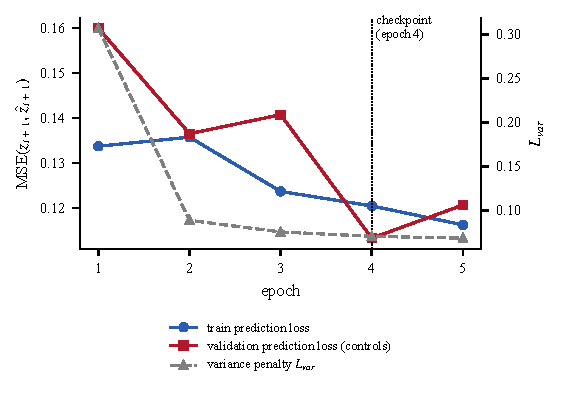
\includegraphics[width=\columnwidth]{figures/fig_training.pdf}
\caption{Training curves (5 epochs, train-control subjects). Source: \texttt{training\_report.json}.}
\label{fig:training}
\end{figure}

\begin{figure*}[!tp]
\centering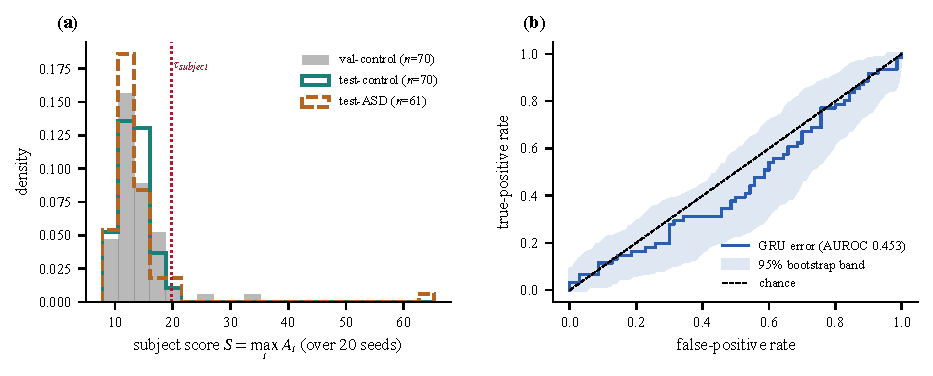
\includegraphics[width=\textwidth]{figures/fig_phase1.pdf}
\caption{Detector test results. (a) Subject scores (maximum over 20 seeds and transitions) for validation controls, test controls and test ASD subjects, with $\tau_{subject}$ (19.81). (b) ROC curve on the 131 test subjects with a 95\% bootstrap band.}
\label{fig:phase1}
\end{figure*}

\begin{figure}[!tbp]
\centering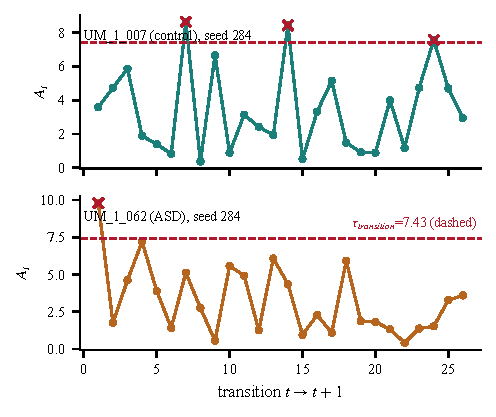
\includegraphics[width=\columnwidth]{figures/fig_timeline.pdf}
\caption{Transition scores $A_t$ for seed ROI 284 of two real test subjects (one control, one ASD) with $\tau_{transition}$ (dashed) and exceedances (crosses). The two subjects are shown for illustration only and are not representative of group differences.}
\label{fig:timeline}
\end{figure}

\subsection{Baselines for temporal modelling (RQ1)}
Table~\ref{tab:scoring} compares three scoring functions on the same frozen encoder, subjects and aggregation: GRU prediction error; a persistence baseline $\|z^{(k+1)}-z^{(k)}\|_2$ with no learned dynamics; and a static baseline, the standardized distance of $z^{(k)}$ from the per-seed train-control centroid, with no temporal information. The AUROC differences (0.453 vs.\ 0.485 vs.\ 0.452) lie well inside each other's confidence intervals, and none differs from chance. Because the encoder was trained jointly with the GRU, the static and persistence baselines are not independent of the temporal objective. Using the mean rather than the maximum over transitions changed AUROC to 0.471 (GRU), 0.508 (persistence) and 0.455 (static), again within noise. Subject score correlated weakly with the number of windows (Spearman 0.229), and scan length alone had AUROC 0.515 for the label, so length is not driving the lack of separation. Whole-graph baselines were not trained (RQ2).

\begin{table*}[!tp]
\caption{Scoring-function comparison on the 131 test subjects (frozen encoder; subject score = max over seeds and transitions; threshold = $P_{95}$ of validation-control scores). AUROC with 95\% bootstrap CI and permutation $p$ against 0.5. Prevalence 0.466. Last column: AUROC when the mean over transitions replaces the maximum.}
\label{tab:scoring}
\centering\footnotesize
\begin{tabular}{@{}lcccccccc@{}}
\toprule
Scoring function & AUROC [95\% CI] & $p$ & AUPRC & Prec. & Rec. & F1 & Flagged & AUROC (mean) \\
\midrule
Static subgraph (distance to control centroid) & 0.452 [0.356, 0.553] & 0.34 & 0.489 & 0.556 & 0.082 & 0.143 & 9 & 0.455 \\
Temporal, no learned dynamics (persistence) & 0.485 [0.380, 0.582] & 0.78 & 0.484 & 0.500 & 0.033 & 0.062 & 4 & 0.508 \\
Temporal, GRU prediction error (ours) & 0.453 [0.353, 0.552] & 0.35 & 0.467 & 0.500 & 0.033 & 0.062 & 4 & 0.471 \\

Whole-graph static / temporal & \multicolumn{8}{c}{not evaluated (no whole-graph encoder was trained)} \\
\bottomrule
\end{tabular}
\end{table*}

\subsection{Generated anomalies}
The generator produced 7,200 records (60 train-control subjects, 20 seeds, 3 severities, 2 methods) in 79~s. Range and finiteness were checked on every record (0 violations); symmetry, unchanged node/edge sets and the absence of self-loops hold by construction and are unit-tested. Mean score after generation rose monotonically with severity for structure-aware edits (4.02, 5.82, 7.63 at $\alpha=0.25,0.55,0.9$) and was flat for random edits (2.91, 2.88, 2.84; Fig.~\ref{fig:phase2}a). The score increased in 99.4--99.6\% of structure-aware records versus 44.8--47.6\% of random records (median change +4.41 vs.\ $-0.07$ at $\alpha=0.9$). Against $\tau_{tr}$, 45.8\% of structure-aware/high transitions exceeded it, versus 4.8\% for random/high, 7.8\% and 23.0\% for structure-aware low/medium, and 5.0\% and 4.9\% for real validation-control and real test-ASD transitions (Fig.~\ref{fig:phase2}b): a 9.6-fold difference. Mean pairwise Jaccard distance between modified-edge sets was 0.999--1.000. At $\alpha=0.9$ an average of 104.8 edge pairs were edited per record. Two caveats apply. The edit maximizes the same model's error, so the effect is expected by construction and is not independent evidence of biological plausibility; and real ASD transitions are exceeded at the control rate (4.9\% vs.\ 5.0\%), i.e.\ synthetic anomalies are far larger deviations than any real group difference found here.

\begin{figure*}[!tp]
\centering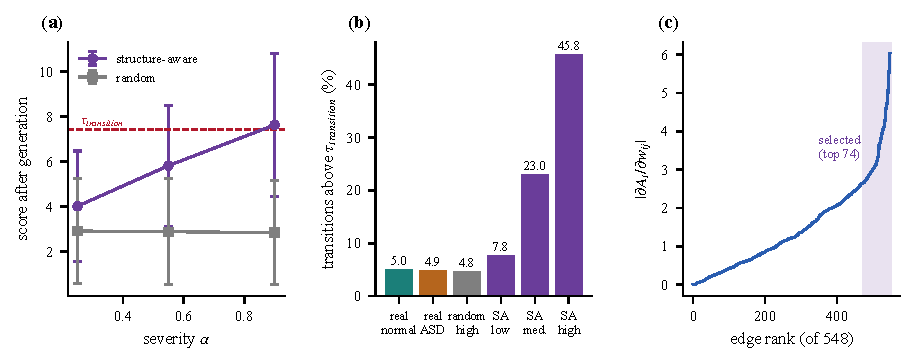
\includegraphics[width=\textwidth]{figures/fig_phase2.pdf}
\caption{Anomaly generation. (a) Score after generation vs.\ severity (mean $\pm$ SD over 1,200 records per point). (b) Fraction of transitions above $\tau_{transition}$ (SA = structure-aware). (c) Sorted gradient sensitivity for one real record (KKI\_002, seed 1) with the selected 74 of 548 edge pairs.}
\label{fig:phase2}
\end{figure*}

\subsection{Few-shot evaluation (RQ3)}
Table~\ref{tab:fewshot} and Fig.~\ref{fig:phase3} give the five-draw results. With one real ASD subject the head almost never flags anyone (F1 0.006, recall 0.003); adding 30 generated anomalies of either type raises 1-shot F1 to 0.39 (structure-aware) and 0.40 (random). Recall rises correspondingly, but AUROC and AUPRC stay between 0.47 and 0.52 in every condition. The F1 gain is explained by the flag rate: the adapted heads flag 35--39\% of test subjects at precision close to the prevalence, and a prevalence-matched random flagger at the same rate would obtain F1 0.40--0.42 (Table~\ref{tab:fewshot}, last column). Paired over draws, structure-aware minus random changed F1 by $-0.017$, $-0.009$, $-0.029$ (1, 5, 10 shots; ranges span zero) and AUROC by $-0.009$, $-0.015$, $-0.013$ (1, 5, 10 shots; ranges also span zero), so there is no evidence that structure-aware generation is better than random here, despite the 9.6-fold difference in the generation analysis. We hypothesize, without testing it, that each generated vector changes only one of 20 dimensions, which gives a linear classifier little per-dimension signal.

\begin{table*}[!tp]
\caption{Few-shot comparison on the 131 test subjects (mean $\pm$ SD over five support-set draws, shared test set). ``Flag'' is the mean fraction of test subjects flagged; $F1_{chance}$ is the F1 of a prevalence-matched random classifier flagging the same fraction. n/a: not derivable (precision or recall is zero in some draws).}
\label{tab:fewshot}
\centering\footnotesize
\setlength{\tabcolsep}{3pt}
\begin{tabular}{@{}clccccccc@{}}
\toprule
$k$ & Condition & Precision & Recall & F1 & AUROC & AUPRC & Flag & $F1_{chance}$ \\
\midrule
\multirow{3}{*}{1} & Few-shot only & 0.200$\pm$0.40 & 0.003$\pm$0.01 & 0.006$\pm$0.01 & 0.516$\pm$0.06 & 0.489$\pm$0.05 & n/a & n/a \\
 & + structure-aware & 0.443$\pm$0.05 & 0.344$\pm$0.04 & 0.387$\pm$0.04 & 0.497$\pm$0.03 & 0.470$\pm$0.05 & 0.36 & 0.41 \\
 & + random & 0.473$\pm$0.04 & 0.357$\pm$0.09 & 0.403$\pm$0.07 & 0.506$\pm$0.04 & 0.487$\pm$0.03 & 0.35 & 0.40 \\
\midrule
\multirow{3}{*}{5} & Few-shot only & 0.430$\pm$0.13 & 0.092$\pm$0.04 & 0.149$\pm$0.07 & 0.485$\pm$0.02 & 0.466$\pm$0.02 & 0.10 & 0.16 \\
 & + structure-aware & 0.447$\pm$0.02 & 0.348$\pm$0.04 & 0.390$\pm$0.03 & 0.486$\pm$0.03 & 0.474$\pm$0.04 & 0.36 & 0.41 \\
 & + random & 0.451$\pm$0.03 & 0.361$\pm$0.06 & 0.399$\pm$0.05 & 0.502$\pm$0.02 & 0.483$\pm$0.02 & 0.37 & 0.41 \\
\midrule
\multirow{3}{*}{10} & Few-shot only & 0.433$\pm$0.07 & 0.249$\pm$0.09 & 0.311$\pm$0.09 & 0.524$\pm$0.05 & 0.486$\pm$0.03 & 0.26 & 0.33 \\
 & + structure-aware & 0.445$\pm$0.05 & 0.367$\pm$0.05 & 0.402$\pm$0.05 & 0.501$\pm$0.05 & 0.481$\pm$0.05 & 0.38 & 0.42 \\
 & + random & 0.474$\pm$0.03 & 0.400$\pm$0.06 & 0.431$\pm$0.04 & 0.515$\pm$0.05 & 0.473$\pm$0.03 & 0.39 & 0.42 \\
\bottomrule

\end{tabular}
\end{table*}

\begin{figure*}[!tp]
\centering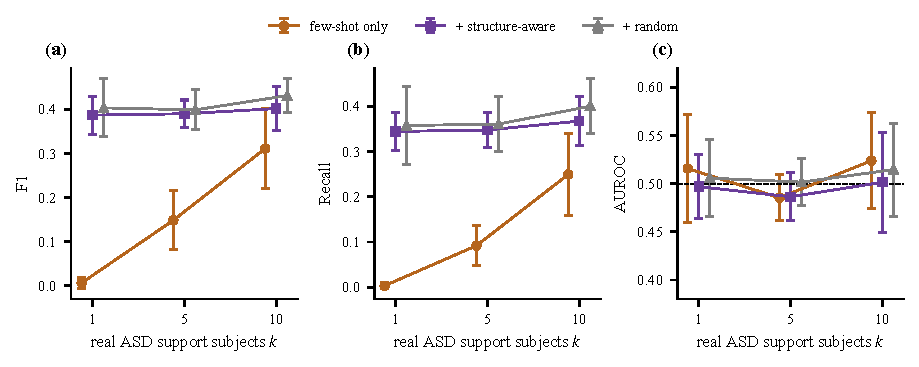
\includegraphics[width=\textwidth]{figures/fig_phase3.pdf}
\caption{Few-shot results (mean $\pm$ SD over five support draws) for (a) F1, (b) recall and (c) AUROC; the dashed line marks chance AUROC.}
\label{fig:phase3}
\end{figure*}

\subsection{Recurrence and reproducibility (RQ4)}
Following Eq.~(\ref{eq:recurrence}), mean recurrence was 0.550$\pm$0.207, 0.512$\pm$0.105 and 0.459$\pm$0.040 for 1, 5 and 10 support subjects. These values are uninformative without a null: on held-out controls (validation plus test controls, $n{=}140$) the mean fraction of seeds with at least one transition above $\tau_{tr}$ was 0.488 (95\% CI 0.459--0.516), against 0.498 (0.476--0.520) for the 281 train-ASD subjects (Mann--Whitney $p{=}0.50$); per-transition exceedance was 5.09\% vs.\ 5.01\%. Across the 20 seeds, one (ROI 109; 0.36 vs.\ 0.53) reached Bonferroni-adjusted significance ($p{=}0.0019$ against a threshold of 0.0025); with 20 tests this is an exploratory observation that needs independent confirmation. Rankings of seeds by recurrence were nearly uncorrelated between independent support draws (mean pairwise Spearman 0.04, 0.07, 0.13 for 1, 5, 10 shots). Recurring anomalous subgraphs are therefore not reproducible in the present configuration.

\subsection{Severity estimation (RQ7)}
On the 60 validation and test ASD subjects with CSS, the severity classifier reached accuracy 0.433 and macro-F1 0.395, below the 0.550 obtained by always answering ``high'' (Table~\ref{tab:severity}). Across repeated 5-fold cross-validation over all 193 subjects, accuracy was $0.391\pm0.066$ against 0.430 for the majority rule; macro-F1 0.372 was not significantly above permuted labels ($p{=}0.080$). The regression analogue showed no association between predicted and true CSS (Spearman 0.131, $p{=}0.32$), and the detector's subject score was uncorrelated with CSS across the 193 subjects (Spearman 0.046, $p{=}0.52$). The scores therefore carry no usable severity information in this configuration. Because the detector flags almost no one (Sec.~VII-A), the severity estimator is also rarely invoked in the application.

\begin{table}[!tbp]
\caption{Severity-band estimation (3 classes: low, moderate, high). Majority-class accuracy is the accuracy of always predicting the most common training band; uniform chance is 0.333.}
\label{tab:severity}
\centering\footnotesize
\begin{tabular}{@{}lcccc@{}}
\toprule
Evaluation & $n$ & Accuracy & Macro-F1 & Majority \\
\midrule
Held-out (val.\ + test ASD) & 60 & 0.433 & 0.395 & 0.550 \\
5-fold CV $\times$10 (all) & 193 & 0.391$\pm$0.066 & 0.372 & 0.430 \\
\bottomrule
\end{tabular}
\end{table}

\subsection{Ablation coverage and computational cost}
Table~\ref{tab:ablation} states which component contributions were isolated. Training took 299.7~s (6,560 sequences/epoch, 5 epochs); detector evaluation took 27~s; generating the 7,200 records took 79~s and the 45 few-shot classifier fits with scoring 86~s; extracting all 360 seeds costs 71.5~s per subject and peak memory was 98.5~MB (Table~\ref{tab:cost}).

\begin{table}[!tbp]
\caption{Component ablation and coverage.}
\label{tab:ablation}
\centering\footnotesize
\setlength{\tabcolsep}{3pt}
\begin{tabular}{@{}p{2.25cm}p{3.6cm}p{1.7cm}@{}}
\toprule
Component & Comparison and outcome & Status \\
\midrule
Temporal model & GRU vs.\ persistence vs.\ static: AUROC 0.453 / 0.485 / 0.452, CIs overlap & evaluated \\
Subgraph localization & vs.\ whole-graph scoring & not evaluated \\
GIN encoder & alternative encoders & not evaluated \\
Variance term & $\lambda{=}0$ & not evaluated \\
Generated anomalies & F1 up, AUROC unchanged; $F1\approx F1_{chance}$ & evaluated \\
Structure-aware vs.\ random & Generation: 45.8\% vs.\ 4.8\%; few-shot: no gain & evaluated \\
Recurrence & ASD 0.498 vs.\ control 0.488 flagged seeds & evaluated \\
Severity estimation & Accuracy 0.433 vs.\ majority 0.550 & evaluated \\
Support-weighted score & $A(1{+}\lambda C)$ & not implemented \\
\bottomrule
\end{tabular}
\end{table}

\begin{table}[!tbp]
\caption{Computational cost (Apple-silicon laptop; GPU via PyTorch MPS except cache build on CPU).}
\label{tab:cost}
\centering\footnotesize
\begin{tabular}{@{}p{4.1cm}p{3.7cm}@{}}
\toprule
Stage & Measured \\
\midrule
Cache 20 seeds, 871 subjects (CPU) & 112 s \\
Joint training (5 epochs) & 299.7 s \\
Detector evaluation and localization & 27 s \\
Generate 7,200 records & 79 s \\
45 few-shot fits + scoring & 86 s \\
All-360-seed extraction & 71.5 s/subject; 98.5 MB peak \\
\bottomrule
\end{tabular}
\end{table}

%=====================================================================
\FloatBarrier
\section{DISCUSSION}
\label{sec:discussion}
\textbf{Answers to the research questions.} RQ1 (temporal modelling): not supported; GRU, persistence and static scoring are all at chance with overlapping intervals. RQ2 (subgraph vs.\ whole graph): not evaluated. RQ3 (few-shot): partially; F1 and recall rise, but this is accounted for by the flag rate, and ranking performance does not improve. RQ4 (reproducibility): not supported; recurrence is at the control null and its rankings are unstable. RQ5 (robustness to window, sparsification, subgraph size): not evaluated beyond the aggregation check. RQ6 (site generalization): not evaluated; all 20 sites appear in every split. RQ7 (severity): not supported; the estimator is below a majority-class rule and the scores are uncorrelated with CSS.

\textbf{Interpretation.} The most defensible reading is that the pipeline works as an engineering system (stable training without collapse, valid and diverse generated records, a controllable severity dial) but that the learned prediction error does not capture a difference between ASD and control subjects at this scale. Possible causes, none tested here, include the diagnostic label being a weak proxy for abnormal dynamics, heterogeneity of ASD, residual site effects \cite{yu2018harm,abraham2017}, short windows with noisy correlations \cite{hutchison2013}, the small number of train-control sequences, and the use of only 20 of 360 candidate seeds. The detectability of generated anomalies is a property of the generator and the scoring model sharing parameters; it shows the generator is not equivalent to random noise, not that its outputs resemble clinical anomalies.

\textbf{Threats to validity.} (i) Diagnosis as proxy label; (ii) 131 test subjects give wide intervals (AUROC width about 0.2); (iii) no site harmonization; (iv) single training seed, so training variance is unreported; (v) two post-hoc design steps (two thresholds, 20-D features) followed first looks at test outputs; (vi) generated positives in the few-shot head are near-copies of negative-pool vectors with one entry changed, which can inflate flag rate without improving ranking; (vii) the F1 comparison of conditions with different flag rates is not like-for-like, which is why $F1_{chance}$ is reported; (viii) stable tracking fixes ROI membership but not edge presence, and 1-node degenerate subgraphs exist.

\textbf{Implications.} Reporting AUROC, flag rates and chance-matched F1 together avoids over-reading F1 gains in few-shot anomaly detection. Where ground truth for abnormal transitions is unavailable, generated anomalies can validate a scoring function's sensitivity, but they cannot validate its clinical relevance.

%=====================================================================
\section{CONCLUSION AND FUTURE WORK}
We formulated and implemented few-shot temporal subgraph anomaly detection on ABIDE I, with a control-trained GIN+GRU predictor, two-level calibration and a gradient-guided generator of synthetic anomalies. The generator behaves as designed, but the detector does not separate ASD from control subjects (AUROC 0.453, 95\% CI 0.353--0.552), baselines are equally at chance, and few-shot gains in F1 are attributable to flag rate rather than discrimination. Needed next: whole-graph and alternative-encoder baselines; leave-site-out evaluation with harmonization; multiple training seeds; sweeps over window length, sparsification and subgraph size; evaluating generated anomalies with an independent encoder; richer few-shot features (per-window or attention-based); anatomical labelling of flagged ROIs with the Glasser atlas; and, only then, stronger claims. No clinical use is implied.

\balance
\begin{thebibliography}{57}
\bibitem{bullmore2009}
E. Bullmore and O. Sporns, ``Complex brain networks: Graph theoretical analysis of structural and functional systems,'' \emph{Nat. Rev. Neurosci.}, vol. 10, no. 3, pp. 186--198, Mar. 2009, doi: 10.1038/nrn2575.

\bibitem{smith2011}
S. M. Smith \emph{et al.}, ``Network modelling methods for FMRI,'' \emph{NeuroImage}, vol. 54, no. 2, pp. 875--891, Jan. 2011, doi: 10.1016/j.neuroimage.2010.08.063.

\bibitem{dimartino2014}
A. Di Martino \emph{et al.}, ``The autism brain imaging data exchange: Towards a large-scale evaluation of the intrinsic brain architecture in autism,'' \emph{Mol. Psychiatry}, vol. 19, no. 6, pp. 659--667, Jun. 2014, doi: 10.1038/mp.2013.78.

\bibitem{parisot2018}
S. Parisot \emph{et al.}, ``Disease prediction using graph convolutional networks: Application to autism spectrum disorder and Alzheimer's disease,'' \emph{Med. Image Anal.}, vol. 48, pp. 117--130, Aug. 2018, doi: 10.1016/j.media.2018.06.001.

\bibitem{li2021braingnn}
X. Li \emph{et al.}, ``BrainGNN: Interpretable brain graph neural network for fMRI analysis,'' \emph{Med. Image Anal.}, vol. 74, Art. no. 102233, Dec. 2021, doi: 10.1016/j.media.2021.102233.

\bibitem{kan2022}
X. Kan, W. Dai, H. Cui, Z. Zhang, Y. Guo, and C. Yang, ``Brain network transformer,'' in \emph{Adv. Neural Inf. Process. Syst. (NeurIPS)}, vol. 35, 2022.

\bibitem{cui2023}
H. Cui \emph{et al.}, ``BrainGB: A benchmark for brain network analysis with graph neural networks,'' \emph{IEEE Trans. Med. Imag.}, vol. 42, no. 2, pp. 493--506, Feb. 2023, doi: 10.1109/TMI.2022.3218745.

\bibitem{abraham2017}
A. Abraham \emph{et al.}, ``Deriving reproducible biomarkers from multi-site resting-state data: An autism-based example,'' \emph{NeuroImage}, vol. 147, pp. 736--745, Feb. 2017, doi: 10.1016/j.neuroimage.2016.10.045.

\bibitem{heinsfeld2018}
A. S. Heinsfeld, A. R. Franco, R. C. Craddock, A. Buchweitz, and F. Meneguzzi, ``Identification of autism spectrum disorder using deep learning and the ABIDE dataset,'' \emph{NeuroImage Clin.}, vol. 17, pp. 16--23, 2018, doi: 10.1016/j.nicl.2017.08.017.

\bibitem{yu2018harm}
M. Yu \emph{et al.}, ``Statistical harmonization corrects site effects in functional connectivity measurements from multi-site fMRI data,'' \emph{Hum. Brain Mapp.}, vol. 39, no. 11, pp. 4213--4227, Nov. 2018, doi: 10.1002/hbm.24241.

\bibitem{hutchison2013}
R. M. Hutchison \emph{et al.}, ``Dynamic functional connectivity: Promise, issues, and interpretations,'' \emph{NeuroImage}, vol. 80, pp. 360--378, Oct. 2013, doi: 10.1016/j.neuroimage.2013.05.079.

\bibitem{allen2014}
E. A. Allen, E. Damaraju, S. M. Plis, E. B. Erhardt, T. Eichele, and V. D. Calhoun, ``Tracking whole-brain connectivity dynamics in the resting state,'' \emph{Cereb. Cortex}, vol. 24, no. 3, pp. 663--676, Mar. 2014, doi: 10.1093/cercor/bhs352.

\bibitem{preti2017}
M. G. Preti, T. A. Bolton, and D. Van De Ville, ``The dynamic functional connectome: State-of-the-art and perspectives,'' \emph{NeuroImage}, vol. 160, pp. 41--54, Oct. 2017, doi: 10.1016/j.neuroimage.2016.12.061.

\bibitem{kim2021}
B.-H. Kim, J. C. Ye, and J.-J. Kim, ``Learning dynamic graph representation of brain connectome with spatio-temporal attention,'' in \emph{Adv. Neural Inf. Process. Syst. (NeurIPS)}, vol. 34, 2021, arXiv:2105.13495.

\bibitem{gadgil2020}
S. Gadgil, Q. Zhao, A. Pfefferbaum, E. V. Sullivan, E. Adeli, and K. M. Pohl, ``Spatio-temporal graph convolution for resting-state fMRI analysis,'' in \emph{Med. Image Comput. Comput.-Assist. Intervent. (MICCAI)}, 2020, pp. 528--538, doi: 10.1007/978-3-030-59728-3\_52.

\bibitem{marquand2016}
A. F. Marquand, I. Rezek, J. Buitelaar, and C. F. Beckmann, ``Understanding heterogeneity in clinical cohorts using normative models: Beyond case-control studies,'' \emph{Biol. Psychiatry}, vol. 80, no. 7, pp. 552--561, Oct. 2016, doi: 10.1016/j.biopsych.2015.12.023.

\bibitem{ma2023survey}
X. Ma \emph{et al.}, ``A comprehensive survey on graph anomaly detection with deep learning,'' \emph{IEEE Trans. Knowl. Data Eng.}, vol. 35, no. 12, pp. 12012--12038, Dec. 2023, doi: 10.1109/TKDE.2021.3118815.

\bibitem{gotham2009}
K. Gotham, A. Pickles, and C. Lord, ``Standardizing ADOS scores for a measure of severity in autism spectrum disorders,'' \emph{J. Autism Dev. Disord.}, vol. 39, no. 5, pp. 693--705, May 2009, doi: 10.1007/s10803-008-0674-3.

\bibitem{xu2019gin}
K. Xu, W. Hu, J. Leskovec, and S. Jegelka, ``How powerful are graph neural networks?'' in \emph{Proc. Int. Conf. Learn. Represent. (ICLR)}, 2019, arXiv:1810.00826.

\bibitem{cho2014}
K. Cho \emph{et al.}, ``Learning phrase representations using RNN encoder-decoder for statistical machine translation,'' in \emph{Proc. Conf. Empirical Methods Natural Lang. Process. (EMNLP)}, Doha, Qatar, Oct. 2014, pp. 1724--1734, doi: 10.3115/v1/D14-1179.

\bibitem{glasser2016}
M. F. Glasser \emph{et al.}, ``A multi-modal parcellation of human cerebral cortex,'' \emph{Nature}, vol. 536, no. 7615, pp. 171--178, Aug. 2016, doi: 10.1038/nature18933.

\bibitem{ktena2017}
S. I. Ktena \emph{et al.}, ``Distance metric learning using graph convolutional networks: Application to functional brain networks,'' in \emph{Med. Image Comput. Comput.-Assist. Intervent. (MICCAI)}, 2017, pp. 469--477, doi: 10.1007/978-3-319-66182-7\_54.

\bibitem{kawahara2017}
J. Kawahara \emph{et al.}, ``BrainNetCNN: Convolutional neural networks for brain networks; towards predicting neurodevelopment,'' \emph{NeuroImage}, vol. 146, pp. 1038--1049, Feb. 2017, doi: 10.1016/j.neuroimage.2016.09.046.

\bibitem{kipf2017}
T. N. Kipf and M. Welling, ``Semi-supervised classification with graph convolutional networks,'' in \emph{Proc. Int. Conf. Learn. Represent. (ICLR)}, 2017, arXiv:1609.02907.

\bibitem{lanciano2020}
T. Lanciano, F. Bonchi, and A. Gionis, ``Explainable classification of brain networks via contrast subgraphs,'' in \emph{Proc. ACM SIGKDD Int. Conf. Knowl. Discovery Data Mining (KDD)}, 2020, pp. 3308--3318, doi: 10.1145/3394486.3403383.

\bibitem{rossi2020tgn}
E. Rossi, B. Chamberlain, F. Frasca, D. Eynard, F. Monti, and M. Bronstein, ``Temporal graph networks for deep learning on dynamic graphs,'' arXiv:2006.10637, Jun. 2020.

\bibitem{pareja2020}
A. Pareja \emph{et al.}, ``EvolveGCN: Evolving graph convolutional networks for dynamic graphs,'' in \emph{Proc. AAAI Conf. Artif. Intell.}, vol. 34, no. 4, 2020, pp. 5363--5370, doi: 10.1609/aaai.v34i04.5984.

\bibitem{aggarwal2019}
P. Aggarwal and A. Gupta, ``Multivariate graph learning for detecting aberrant connectivity of dynamic brain networks in autism,'' \emph{Med. Image Anal.}, vol. 56, pp. 11--25, Aug. 2019, doi: 10.1016/j.media.2019.05.007.

\bibitem{pang2021review}
G. Pang, C. Shen, L. Cao, and A. van den Hengel, ``Deep learning for anomaly detection: A review,'' \emph{ACM Comput. Surv.}, vol. 54, no. 2, 2022, doi: 10.1145/3439950.

\bibitem{ding2019dominant}
K. Ding, J. Li, R. Bhanushali, and H. Liu, ``Deep anomaly detection on attributed networks,'' in \emph{Proc. SIAM Int. Conf. Data Mining (SDM)}, 2019, pp. 594--602, doi: 10.1137/1.9781611975673.67.

\bibitem{ruff2018}
L. Ruff \emph{et al.}, ``Deep one-class classification,'' in \emph{Proc. Int. Conf. Mach. Learn. (ICML)}, PMLR vol. 80, 2018, pp. 4393--4402.

\bibitem{ma2022glocal}
R. Ma, G. Pang, L. Chen, and A. van den Hengel, ``Deep graph-level anomaly detection by glocal knowledge distillation,'' in \emph{Proc. ACM Int. Conf. Web Search Data Mining (WSDM)}, 2022, pp. 704--714, doi: 10.1145/3488560.3498473.

\bibitem{yu2018netwalk}
W. Yu, W. Cheng, C. C. Aggarwal, K. Zhang, H. Chen, and W. Wang, ``NetWalk: A flexible deep embedding approach for anomaly detection in dynamic networks,'' in \emph{Proc. ACM SIGKDD Int. Conf. Knowl. Discovery Data Mining (KDD)}, 2018, pp. 2672--2681, doi: 10.1145/3219819.3220024.

\bibitem{zheng2019addgraph}
L. Zheng, Z. Li, J. Li, Z. Li, and J. Gao, ``AddGraph: Anomaly detection in dynamic graph using attention-based temporal GCN,'' in \emph{Proc. Int. Joint Conf. Artif. Intell. (IJCAI)}, 2019, pp. 4419--4425, doi: 10.24963/ijcai.2019/614.

\bibitem{behrouz2023}
A. Behrouz and M. Seltzer, ``Anomaly detection in human brain via inductive learning on temporal multiplex networks,'' in \emph{Proc. Mach. Learn. Healthcare Conf.}, PMLR vol. 219, 2023, pp. 50--75.

\bibitem{sadeghian2024}
S. Sadeghian, X. Li, and M. Seltzer, ``HyperBrain: Anomaly detection for temporal hypergraph brain networks,'' arXiv:2410.02087, Oct. 2024.

\bibitem{chatterjee2021}
T. Chatterjee, R. Albert, S. Thapliyal, N. Azarhooshang, and B. DasGupta, ``Detecting network anomalies using Forman-Ricci curvature and a case study for human brain networks,'' \emph{Sci. Rep.}, vol. 11, no. 1, Art. no. 8121, Apr. 2021, doi: 10.1038/s41598-021-87587-z.

\bibitem{wang2021fewshot}
Y. Wang, Q. Yao, J. T. Kwok, and L. M. Ni, ``Generalizing from a few examples: A survey on few-shot learning,'' \emph{ACM Comput. Surv.}, vol. 53, no. 3, Art. no. 63, 2020, doi: 10.1145/3386252.

\bibitem{finn2017}
C. Finn, P. Abbeel, and S. Levine, ``Model-agnostic meta-learning for fast adaptation of deep networks,'' in \emph{Proc. Int. Conf. Mach. Learn. (ICML)}, PMLR vol. 70, 2017, pp. 1126--1135.

\bibitem{snell2017}
J. Snell, K. Swersky, and R. Zemel, ``Prototypical networks for few-shot learning,'' in \emph{Adv. Neural Inf. Process. Syst. (NIPS)}, vol. 30, 2017, arXiv:1703.05175.

\bibitem{ding2021fewshot}
K. Ding, Q. Zhou, H. Tong, and H. Liu, ``Few-shot network anomaly detection via cross-network meta-learning,'' in \emph{Proc. Web Conf. (WWW)}, 2021, pp. 2448--2456, doi: 10.1145/3442381.3449922.

\bibitem{pang2019devnet}
G. Pang, C. Shen, and A. van den Hengel, ``Deep anomaly detection with deviation networks,'' in \emph{Proc. ACM SIGKDD Int. Conf. Knowl. Discovery Data Mining (KDD)}, 2019, pp. 353--362, doi: 10.1145/3292500.3330871.

\bibitem{yang2022meta}
Y. Yang \emph{et al.}, ``Data-efficient brain connectome analysis via multi-task meta-learning,'' in \emph{Proc. ACM SIGKDD Int. Conf. Knowl. Discovery Data Mining (KDD)}, 2022, pp. 4743--4751, doi: 10.1145/3534678.3542680.

\bibitem{wei2025}
X. Wei, K. Zhao, Y. Jiao, L. He, and Y. Zhang, ``A brain graph foundation model: Pre-training and prompt-tuning across broad atlases and disorders,'' arXiv:2506.02044, 2025.

\bibitem{dhinagar2023}
N. J. Dhinagar, V. Santhalingam, K. E. Lawrence, E. Laltoo, and P. M. Thompson, ``Few-shot classification of autism spectrum disorder using site-agnostic meta-learning and brain MRI,'' in \emph{Proc. Annu. Int. Conf. IEEE Eng. Med. Biol. Soc. (EMBC)}, 2023, doi: 10.1109/EMBC40787.2023.10340852.

\bibitem{zhao2021smote}
T. Zhao, X. Zhang, and S. Wang, ``GraphSMOTE: Imbalanced node classification on graphs with graph neural networks,'' in \emph{Proc. ACM Int. Conf. Web Search Data Mining (WSDM)}, 2021, pp. 833--841, doi: 10.1145/3437963.3441720.

\bibitem{chen2020gaan}
Z. Chen, B. Liu, M. Wang, P. Dai, J. Lv, and L. Bo, ``Generative adversarial attributed network anomaly detection,'' in \emph{Proc. ACM Int. Conf. Inf. Knowl. Manage. (CIKM)}, 2020, pp. 1989--1992, doi: 10.1145/3340531.3412070.

\bibitem{zugner2018}
D. Z{\"u}gner, A. Akbarnejad, and S. G{\"u}nnemann, ``Adversarial attacks on neural networks for graph data,'' in \emph{Proc. ACM SIGKDD Int. Conf. Knowl. Discovery Data Mining (KDD)}, 2018, pp. 2847--2856, doi: 10.1145/3219819.3220078.

\bibitem{dai2018}
H. Dai \emph{et al.}, ``Adversarial attack on graph structured data,'' in \emph{Proc. Int. Conf. Mach. Learn. (ICML)}, PMLR vol. 80, 2018, pp. 1115--1124.

\bibitem{xu2019topology}
K. Xu \emph{et al.}, ``Topology attack and defense for graph neural networks: An optimization perspective,'' in \emph{Proc. Int. Joint Conf. Artif. Intell. (IJCAI)}, 2019, pp. 3961--3967, doi: 10.24963/ijcai.2019/550.

\bibitem{madry2018}
A. Madry, A. Makelov, L. Schmidt, D. Tsipras, and A. Vladu, ``Towards deep learning models resistant to adversarial attacks,'' in \emph{Proc. Int. Conf. Learn. Represent. (ICLR)}, 2018, arXiv:1706.06083.

\bibitem{brahim2020}
A. Brahim and N. Farrugia, ``Graph Fourier transform of fMRI temporal signals based on an averaged structural connectome for the classification of neuroimaging,'' \emph{Artif. Intell. Med.}, vol. 106, Art. no. 101870, 2020, doi: 10.1016/j.artmed.2020.101870.

\bibitem{abraham2014}
A. Abraham \emph{et al.}, ``Machine learning for neuroimaging with scikit-learn,'' \emph{Front. Neuroinform.}, vol. 8, Art. no. 14, 2014, doi: 10.3389/fninf.2014.00014.

\bibitem{bardes2022}
A. Bardes, J. Ponce, and Y. LeCun, ``VICReg: Variance-invariance-covariance regularization for self-supervised learning,'' in \emph{Proc. Int. Conf. Learn. Represent. (ICLR)}, 2022, arXiv:2105.04906.

\bibitem{paszke2019}
A. Paszke \emph{et al.}, ``PyTorch: An imperative style, high-performance deep learning library,'' in \emph{Adv. Neural Inf. Process. Syst. (NeurIPS)}, vol. 32, 2019, arXiv:1912.01703.

\bibitem{fey2019}
M. Fey and J. E. Lenssen, ``Fast graph representation learning with PyTorch Geometric,'' in \emph{ICLR Workshop Representation Learn. Graphs Manifolds}, 2019, arXiv:1903.02428.

\bibitem{kingma2015}
D. P. Kingma and J. Ba, ``Adam: A method for stochastic optimization,'' in \emph{Proc. Int. Conf. Learn. Represent. (ICLR)}, 2015, arXiv:1412.6980.

\end{thebibliography}


\end{document}
